
\section{Patrones de diseño}
Un patrón de diseño es: \cite{patrondiseno}\\
\begin{itemize}
    \item una solución estándar para un problema común de programación
    \item una técnica para flexibilizar el código haciéndolo satisfacer ciertos criterios
    \item un proyecto o estructura de implementación que logra una finalidad determinada
    \item un lenguaje de programación de alto nivel
    \item una manera más práctica de describir ciertos aspectos de la organización de un programa
    \item conexiones entre componentes de programas
    \item la forma de un diagrama de objeto o de un modelo de objeto.
\end{itemize}
 

\subsection{Patrón de diseño Modelo Vista Controlador (MVC)}
Es un patrón de arquitectura de las aplicaciones software.\\ 
\begin{itemize}
    \item Separa la lógica de negocio de la interfaz de usuario
    \item Facilita la evolución por separado de ambos aspectos
    \item Incrementa reutilización y flexibilidad
\end{itemize}

Descrito por primera vez en 1979 para Smalltalk y posteriormente utilizado en múltiples frameworks como: 
\begin{itemize}
    \item Java Swing
    \item Java Enterprise Edition (J2EE)
    \item XForms (Formato XML estándar del W3C para la especificación de un modelo de proceso de datos XML e interfaces de usuario como formularios web)
    \item GTK+ (escrito en C, toolkit creado por Gnome para construir aplicaciones gráficas, inicialmente para el sistema X Window)
    \item ASP.NET MVC Framework (Microsoft)
    \item Google Web Toolkit (GWT, para crear aplicaciones Ajax con Java)
    \item Apache Struts (framework para aplicaciones web J2EE)
    \item Ruby on Rails (framework para aplicaciones web con Ruby)
\end{itemize}

Modelo-Vista-Controlador
\begin{itemize}
    \item Un modelo
    \item Varias vistas
    \item Varios controladores
\end{itemize}

Las vistas y los controladores suelen estar muy relacionados, los controladores tratan los eventos que se producen en la
interfaz gráfica (vista)

Esta separación de aspectos de una aplicación da mucha
flexibilidad al desarrollador \cite{mvc}

\begin{figure}[H]
\centering
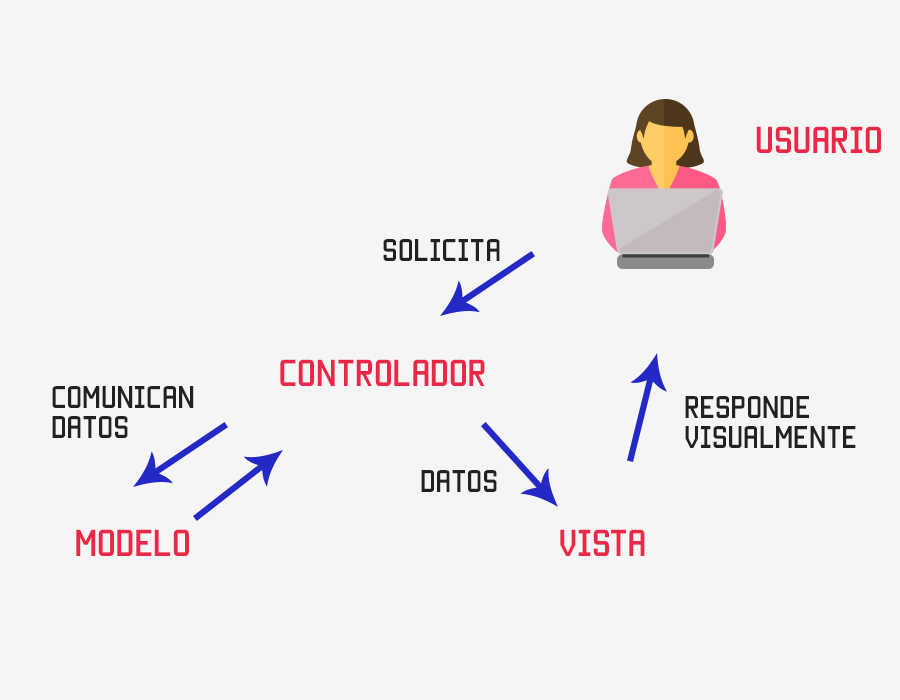
\includegraphics[width=0.75\textwidth]{imagenes/mvc}
\caption{Modelo Vista Controlador}
\label{img:mvc}
\end{figure}

\subsubsection{Modelo}
Se encarga de los datos, generalmente (pero no obligatoriamente) consultando la base de datos. Actualizaciones, consultas, búsquedas, etc. todo eso va aquí, en el modelo. \cite{mvc2}
\\\newline
\subsubsection{Vista}
Son la representación visual de los datos, todo lo que tenga que ver con la interfaz gráfica va aquí. Ni el modelo ni el controlador se preocupan de cómo se verán los datos, esa responsabilidad es únicamente de la vista. \cite{mvc2}
\\\newline
\subsubsection{Controlador}
Se encarga de... controlar, recibe las órdenes del usuario y se encarga de solicitar los datos al modelo y de comunicárselos a la vista. \cite{mvc2}
\\\newline



